\documentclass[a4paper,11pt]{article}

\usepackage[utf8]{inputenc}
\usepackage[T2A]{fontenc}
\usepackage[russian]{babel}
\usepackage{PTSans}
\renewcommand{\familydefault}{\sfdefault}
\usepackage{geometry}
\usepackage{graphicx}
\usepackage{xcolor}
\usepackage{hyperref}
\usepackage{multicol}

\geometry{top=1.0cm, bottom=1.0cm, left=1.4cm, right=1.4cm}

\definecolor{linkblue}{HTML}{4675D5}

\hypersetup{
  colorlinks=true,
  linkcolor=linkblue,
  urlcolor=linkblue,
  pdfborder={0 0 0}
}

\setlength{\parindent}{0pt}
\setlength{\parskip}{0pt}
\setlength{\columnsep}{16pt}

\newlength{\cvsectionsep}
\setlength{\cvsectionsep}{2.5pt}

\newcommand{\cvsection}[1]{%
  \vspace{3pt}%
  \noindent
  \begin{minipage}{\linewidth}
    \hrule height 0.4pt
    \vspace{\cvsectionsep}
    \hbox to \linewidth{\textbf{\MakeUppercase{#1}}\hss}
    \vspace{\cvsectionsep}
    \hrule height 0.4pt
  \end{minipage}%
  \par\vspace{2pt}%
}

\newcommand{\cvskill}[2]{%
  {\raggedright\noindent\textbf{#1} #2\par}
}

\newcommand{\cvprojecttitle}[2]{%
  \vspace{1pt}%
  \noindent\textbf{\MakeUppercase{#1}}\hfill\href{#2}{\textcolor{linkblue}{ссылка}}\par
  \vspace{0.5pt}%
}

\newcommand{\cvprojectbody}[2]{%
  \noindent #1\par
  \vspace{0.5pt}%
  \noindent\textbf{Стек:} #2\par
  \vspace{1pt}%
}

\newcommand{\cvproject}[4]{%
  \cvprojecttitle{#1}{#2}%
  \cvprojectbody{#3}{#4}%
}

\newcommand{\cvjob}[3]{%
  \vspace{1pt}%
  \noindent\textbf{\MakeUppercase{#1}}\par
  \vspace{0.5pt}%
  \noindent\textbf{Место:} #2\par
  \noindent\textbf{Задачи:} #3\par
  \vspace{1pt}%
}

\newcommand{\cvpractice}[3]{%
  \vspace{2pt}%
  \noindent\textbf{#1}\par
  #2\par
  #3\par
  \vspace{3pt}%
}

\newcommand{\cvheader}{%
  \noindent
  \begin{minipage}[t]{0.72\textwidth}
    \vspace{0pt}%
    {\fontsize{16}{18}\selectfont\textbf{БЕЛЯКОВА АННА СТАНИСЛАВОВНА}}\par
    \vspace{4pt}
    \textbf{АНАЛИТИК}\par
    \vspace{30pt}
    +79877288420\,|\,20.07.2005\,|\,\href{https://t.me/belyak_anya}{t.me/belyak\_anya}\par
    belyakova.anna.st@yandex.ru\,|\,\href{https://github.com/belyakova-anna}{github}\,|\,\href{https://www.linkedin.com/in/belyak-anya/}{linkedin}\par
  \end{minipage}%
  \hfill
  \begin{minipage}[t]{0.22\textwidth}
    \vspace{0pt}%
    \raggedleft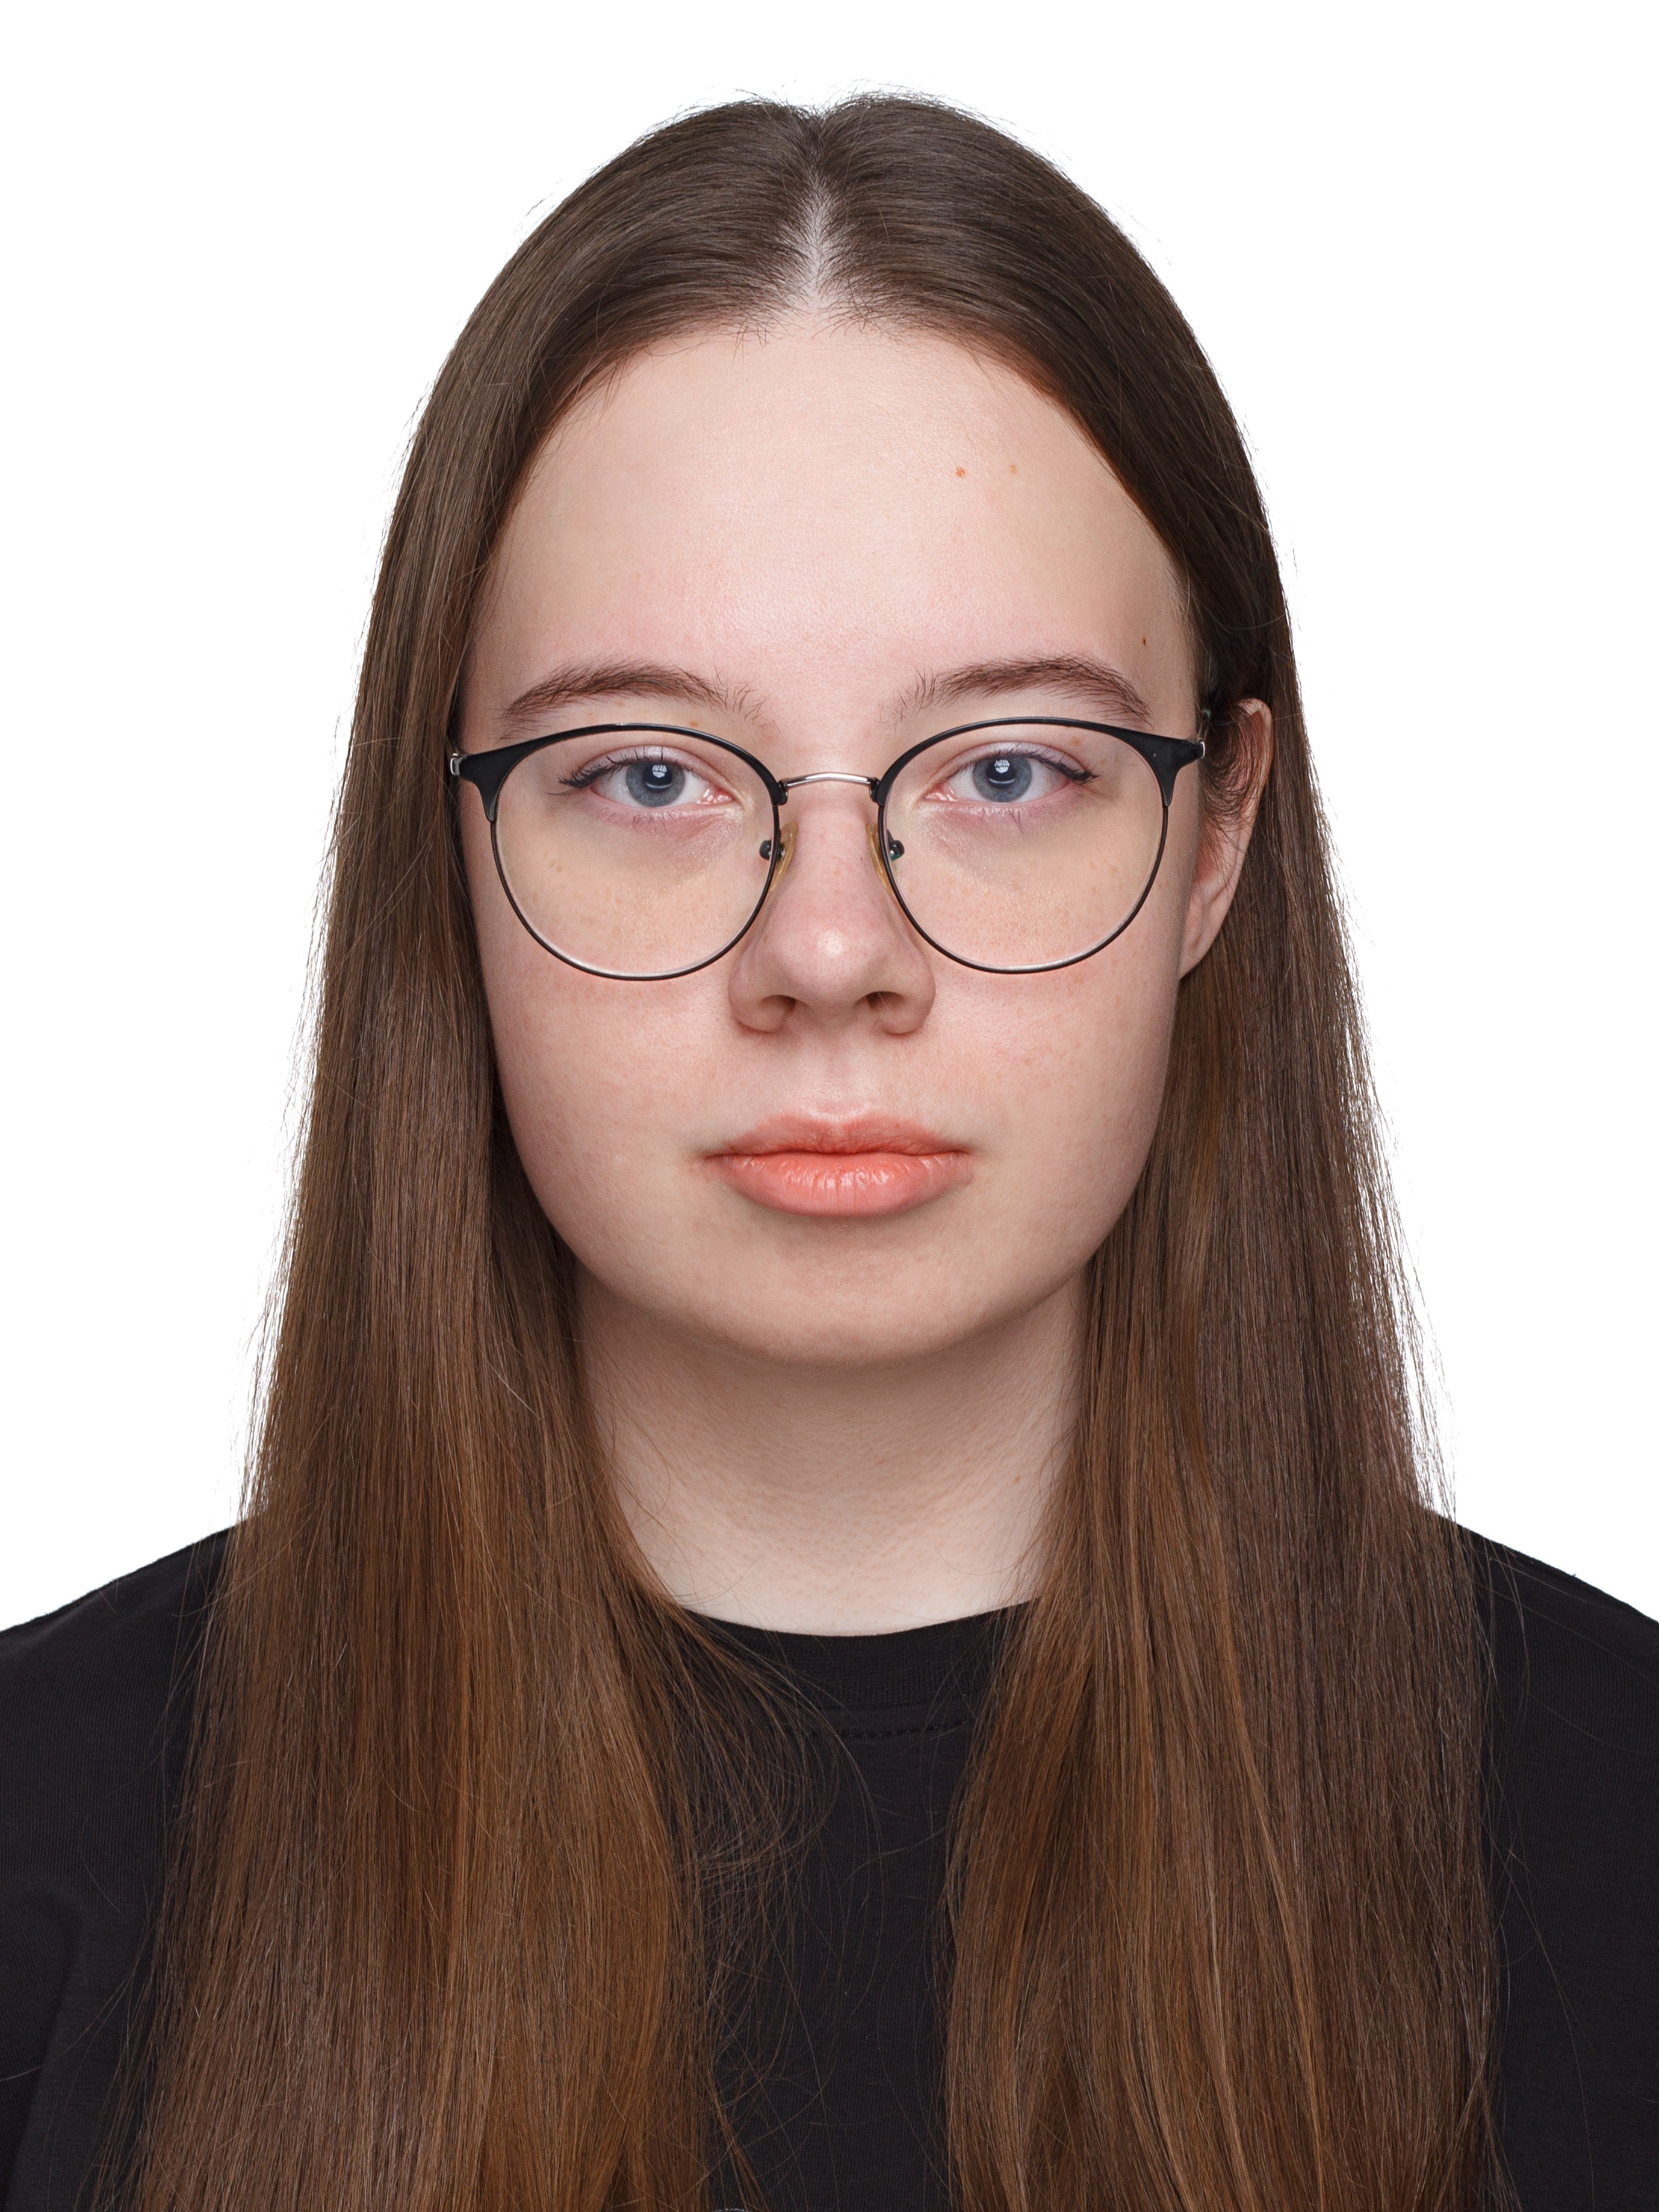
\includegraphics[width=0.6\linewidth]{photo.jpg}
  \end{minipage}%
  \par\vspace{8pt}%
}

\begin{document}
\pagestyle{empty}

\cvheader
\vspace{4pt}

\begin{multicols*}{2}
\linespread{0.93}\selectfont

\cvsection{Образование}

\noindent\textbf{Университет Иннополис}\hfill 2023--2027\par
\vspace{2pt}
\noindent{бакалавриат «Анализ данных и искусственный интеллект».}\par
\vspace{2pt}
\noindent -- средний балл 4.82.\par
\noindent -- обучение на английском языке (уровень Upper-Intermediate).\par
\vspace{4pt}
\noindent\textbf{Deep Learning School}\hfill 2024\par
\noindent{дополнительное образование (машинное обучение).}\par

\cvsection{Навыки}

\cvskill{SQL и базы данных:}{PostgreSQL, MySQL, MongoDB, Neo4j, оконные функции, оптимизация запросов.}
\cvskill{Python и анализ данных:}{pandas, numpy, scipy, scikit-learn, matplotlib.}
\cvskill{Разработка:}{Python (FastAPI), React, C++.}
\cvskill{Статистика и эксперименты:}{теория вероятностей, оценка параметров, доверительные интервалы, A/B тесты, когортный анализ.}
\cvskill{Продуктовая аналитика:}{дерево метрик, целевые метрики, воронки, конверсия, retention, KPI.}
\cvskill{BI и визуализация:}{дашборды, Superset, Python-визуализация, D3.js.}
\cvskill{ETL и данные:}{Airflow, Spark SQL, PySpark, парсинг данных, витрины.}
\cvskill{AI и ML:}{machine learning, computer vision, NLP, RAG, prompt engineering, LangChain.}
\cvskill{DevOps и инструменты:}{Git, Docker, Linux, CI/CD, Jira, Confluence, Miro.}
\cvskill{Анализ и проектирование:}{сбор требований, Use Cases, User Story, BPMN, UML, Scrum, Kanban.}

\cvsection{Опыт работы}

\cvjob{Системный аналитик}{%
  \href{https://t1.ru/about/units/t1-innotech}{Т1 Иннотех}, июль 2026~--- наст. время.}{%
  настраивала Airflow-пайплайны, оптимизировала запросы к базе данных и писала сложные SQL-запросы.}

\cvjob{Продуктовый аналитик}{%
  \href{https://github.com/one-zero-eight}{one-zero-eight}, окт. 2024 г.~--- июль 2026.}{%
  общалась со стейкхолдерами проектов, формализовала требования и следила за прогрессом разработки. Курировала 10+ сервисов на 1500+ постоянных пользователей.}

\cvjob{Специалист}{%
  \href{https://innopolis.university/}{Университет Иннополис}, окт. 2024~-- окт. 2025.}{%
  возглавила процесс автоматизации составления расписания занятий в университете. Ручной труд был заменён на программу, что сократило время составления расписания и практически исключило ошибки.}

\newcolumn

\cvsection{Проекты}

\cvproject{Продуктовая аналитика вебсайта}{https://innohassle.ru/}{%
  разобрала ключевые пользовательские сценарии сайта, структурировала проблемы и предложения по улучшению пользовательского опыта, подготовила основу для приоритизации задач по влиянию на пользователей.}{%
  BPMN, MoSCoW, User Story, CJM, Miro.}

\cvproject{Прогнозирование тяжести ДТП}{https://github.com/Big-Data-IU/US-Accidents}{%
  построила витрины и big data пайплайн для 7.7 млн записей, провела SQL-анализ факторов ДТП и подготовила ML-прогноз тяжести происшествий.}{%
  PostgreSQL, HDFS, Hive, Spark SQL, PySpark MLlib, Superset, Python.}

\cvproject{Анализ рынка вакансий}{https://github.com/belyakova-anna/Statistics-of-requirements-in-IT-vacancies}{%
  собрала вакансии с hh.ru, очистила данные и визуализировала спрос на навыки, зарплаты и роли на IT-рынке Казани.}{%
  Python, парсинг данных, D3.js, визуализация.}

\cvproject{Анализ типа личности}{https://github.com/belyakova-anna/Extrovert-vs.-Introvert-Predictor-Part-2}{%
  подготовила данные, проверила признаки, обучила ML-модель и автоматизировала пайплайн предсказаний.}{%
  Python, pandas, scikit-learn, Airflow.}

\cvproject{Агрегация товаров}{https://github.com/one-zero-eight/hackathon-tenderhack}{%
  кластеризовала товарные позиции и объединила дубли в карточки продуктов для упрощения закупочной аналитики.}{%
  Python, embeddings, AgglomerativeClustering, Qdrant.}

\cvsection{Хакатоны}

\noindent\href{https://drive.google.com/file/d/1jkN7tX9rNNIsZIB6O6MDiqZsnLEl27lU/view?usp=sharing}{\textcolor{linkblue}{Победитель}} хакатона Tender Hack Казань\par
\noindent\href{https://drive.google.com/file/d/1EoGAExuRGV5qIiCAShXfYlCXQAhdUN0J/view?usp=sharing}{\textcolor{linkblue}{Призёр}} хакатона Tender Hack Санкт-Петербург\par
\noindent\href{https://drive.google.com/file/d/1BWFGwSSAwSdn6s5EZF81ADpFYrGgGW7c/view?usp=sharing}{\textcolor{linkblue}{Призёр}} хакатона Архипелаг\par
\noindent Участник: \href{https://drive.google.com/file/d/1F9VDEHMKZnxWCKisxFfVjK9pFhIeqrVx/view?usp=sharing}{Внедрейд}, \href{https://drive.google.com/file/d/1qB8kDuc\_pAsapLfi0IzUPYvbemiUm92D/view?usp=sharing}{True Tech Hack}, \href{https://drive.google.com/file/d/16w7wOoZbr\_ehW2p4fDqZiwhhCTPKn453/view?usp=sharing}{VTB More Tech}, \href{https://drive.google.com/file/d/1rXyqXFqTrNMfYjYB09TvNKFCe8gF2RKY/view?usp=sharing}{Tender Hack Пермь}\par

\cvsection{Достижения}

\noindent\textbf{Член сборной} Республики Татарстан по обработке изображений с БАС\par
\textbf{Член сборной} Республики Марий Эл по спортивному программированию\par
\noindent\textbf{Студент года} Университета Иннополис\par
\textbf{Финалист} Баттла Вузов\par

\end{multicols*}

\end{document}
